
\chapter{\IConfluence and Coordination}
\label{c.iconfluence}

With a system model and goals in hand, we now address the question:
when do applications require coordination for correctness? The answer
depends not just on an application's transactions or on an 
application's invariants. Rather, the answer depends on the
\textit{combination} of the two under consideration. Our contribution
in this section is to formulate a criterion that will answer this
question for specific combinations in an implementation-agnostic
manner.

In this section, we focus almost exclusively on providing a general
answer to this question. The remainder of this thesis is devoted to
practical interpretation and application of these results.

\section{\IConfluence: Criteria Defined}
\label{sec:ic-defs}

To begin, we introduce the central property (adapted from the
constraint programming literature~\cite{obs-confluence}) in our main
result: \iconfluence. Applied in a transactional context, the
\iconfluence property informally ensures that divergent but $I$-valid
database states can be merged into a valid database state---that is,
the set of valid states reachable by executing transactions and
merging their results is closed (w.r.t. validity) under merge. In the
next sub-section, we show that \iconfluence analysis directly
determines the potential for safe, \cfree execution.

We say that a database $D_i$ is a \textit{$I$-$T$-reachable state} if,
given an invariant $I$ and set of transactions $T$ (with merge
function $\sqcup$), there exists a partially ordered set of
transaction and merge function invocations that yields $D_i$, and each
intermediate state produced by transaction execution or merge
invocation is also $I$-valid. We call these previous states
\textit{ancestor states}. Each ancestor state is either the
initial state $D_0$ or is $I$-$T$-reachable from $D_0$.

We can now formalize the \iconfluence property:

\begin{definition}[\IConfluence]
  A set of transactions $T$ is \iconfluent with respect to invariant
  $I$ if, for all $I$-$T$-reachable states $D_i$, $D_j$ with a common
  ancestor state, $D_i \sqcup D_j$ is $I$-valid.
\end{definition}

Figure~\ref{fig:iconfluence} depicts a \iconfluent merge of
two $I$-$T$-reachable states, each starting from a shared,
$I$-$T$-reachable state $D_s$. Two sequences of transactions
$t_{in}\dots t_{i1}$ and $t_{jm}\dots t_{j1}$ each independently
modify $D_s$. Under \iconfluence, the states produced by these
sequences ($D_{in}$ and $D_{jm}$) must be valid under
merge.

We require our merged states in the \iconfluence formulation to have a
common ancestor to rule out the possibility of merging states that
could not have arisen from transaction execution (e.g., even if no
transaction assigns IDs, merging two states that each have unique but
overlapping sets of IDs could be invalid). Moreover, in practice,
every non-\iconfluent set of transactions and invariants we
encountered had a counter-example execution consisting of a divergent
execution consisting of a single pair of transactions. However, we
admit the possiblity that more exotic transactions and merge functions
might lead to complex behavior in non-single-step divergence, so we
consider arbitrary histories here. Precisely characterizing the
difference in expressive power between \iconfluent transactions under
single-transaction divergence versus multi-transaction divergence is
an interesting question for future work.

\Iconfluence holds for specific combinations of invariants and
transactions. In our payroll database example from
Section~\ref{sec:t-motivation}, removing a user from the database is
\iconfluent with respect to the invariant that user IDs are
unique. However, two transactions that remove two different users from
the database are not \iconfluent with respect to the invariant that
there exists at least one user in the database at all times. Later
chapters discuss actual combinations of transactions and invariants
(and with greater precision).

\begin{figure}
\begin{center}
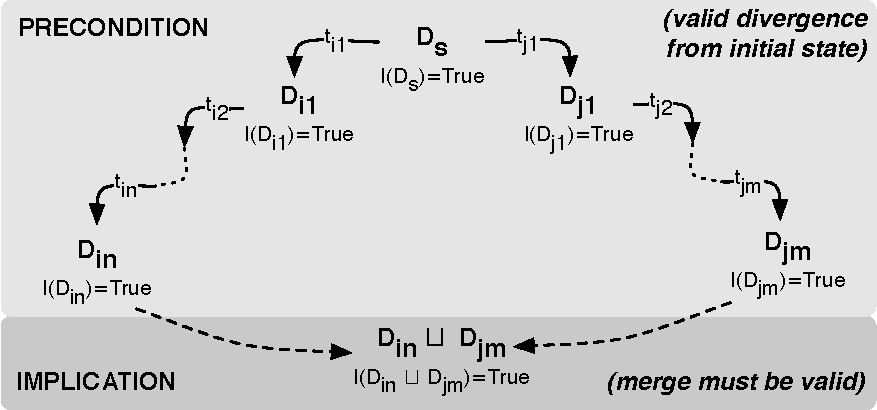
\includegraphics[width=\figscale\columnwidth]{figs/icommute.pdf}\vspace{-1em}
\end{center}\vspace{1em}
\caption{A \iconfluent execution illustrated via a diamond
  diagram. If a set of transactions $T$ is \iconfluent, then all
  database states reachable by executing and merging transactions in
  $T$ starting with a common ancestor ($D_s$) must
  be mergeable ($\sqcup$) into an $I$-valid database state.}
\label{fig:iconfluence}
\end{figure}

\section{\IConfluence and Coordination-Freedom}
\label{sec:ic-result}

We now apply \iconfluence to our goals from Section~\ref{sec:model}:

\begin{theorem}
\label{theorem:necessary}
A globally $I$-valid system can execute a set of transactions $T$ with
\cfreedom, transactional availability, and convergence if and only if $T$
is \iconfluent with respect to $I$.
\end{theorem}

Theorem~\ref{theorem:necessary} establishes \iconfluence as a
necessary and sufficient condition for invariant-preserving,
coordination-free execution.  If \iconfluence holds, there exists a
correct, coordination-free execution strategy for the transactions; if
not, no possible implementation can guarantee these properties for the
provided invariants and transactions. That is, if \iconfluence does
not hold, there exists at least one execution of transactions on
separate replicas that will violate the given invariants when servers
converge. To prevent invalid states from occurring, at least one of
the transaction sequences will have to forego availability or
\cfreedom, or the system will have to forego convergence. \Iconfluence
analysis is independent of any given implementation, and effectively
``lifts'' prior discussions of scalability, availability, and low
latency~\cite{hat-vldb,gilbert-cap,pacelc} to the level of application
(i.e., not ``I/O''~\cite{consistency-borders}) correctness. This
provides a useful handle on the implications of coordination-free
execution without requiring reasoning about low-level properties such
as physical data location and the number of servers.

We provide a full proof of Theorem~\ref{theorem:necessary} below but
first provide a sketch. The backward direction is by construction: if
\iconfluence holds, each replica can check each transaction's
modifications locally and replicas can merge independent modifications
to guarantee convergence to a valid state. The forwards direction uses
a partitioning argument~\cite{gilbert-cap} to derive a contradiction:
we construct a scenario under which a system cannot determine whether
a non-\iconfluent transaction should commit without violating one of
our desired properties (either compromising validity or availability,
diverging forever, or coordinating). The structure of our
argument is not novel, but the ability to discuss the effects of
operations without discussing the underlying system behavior (e.g.,
the presence of network partitions) is useful.

To begin, we demonstrate the possibility of forcing a
coordination-free system into any $I$-$T$-reachable database state via
a carefully crafted sequence of partitioning behavior.

\begin{lemma}\label{lemma:force} 
Given a set of transactions $T$ and invariants $I$, a globally $I$-valid, coordination-free, transactionally available, and convergent system is able to produce any $I$-$T$-reachable state $S_i$.
 \end{lemma}

\begin{proof}[Proof Lemma~\ref{lemma:force}]
Let $\alpha_i$ represent a partially ordered sequence of transactions $T_i$ and merge procedure invocations $M_i$ (call this a \textit{history}) starting from $S_0$ that produces $S_i$.

We $\textsc{replay}$ the history $\alpha$ on a set of servers as
follows. Starting from the initial state $S_0$, we traverse the
partial order according to a topological sort. Initially, we mark all
operations (transactions or merges) in $\alpha$ as \textit{not
  done}. We begin by executing all transactions $T_i$ in $\alpha_i$
that have no predeceding operations in $\alpha$. For each transaction
$t \in T_i$, we execute $t$ on a server that is unable to communicate
with any other server.\footnote{Without loss of generality, we discuss
  replicated databases, where each server contains the entire set of
  items referenced in the history. It is trivial to extend the
  \textsc{replay} procedure to a partially replicated environment by
  replacing each server with a set of servers that contains all data
  items necessary for each operation.} Upon transaction commit, we
merge each replica's modifications into the server.  (Recall that,
because $S_i$ is $I$-$T$-reachable, each transaction in $\alpha$ is an
$I$-valid transformation and must either eventually commit or abort
itself to preserve transactional availability, and, due to
coordination-freedom, the result of the execution is dependent solely
on its input---in this case, $S_0$.) We subsequently mark each
executed transaction $t$ as \textit{done} and denote the server that
executed $t$ as $s_t$.\footnote{Recall from Section~\ref{sec:model}
  that we consider arbitrary groups of servers. Thus, we simply
  execute each operation in the history on a new server. We could be
  more parsimonious with our use of servers in this procedure but
  choose not to do so for simplicity.}

Next, we repeatedly select an operation $o_i$ from $\alpha$ that is
marked as \textit{not done} but whose preceding operations are all
marked as \textit{done}.

If $o_i$ is a transaction with preceding operation $o_j$, performed
corresponding server $s_j$, we \textit{partition} $s_j$, and a second
server $s_i$, a server containing state $S_0$, such that $s_j$ and
$s_i$ can communicate with each other but cannot communicate with any
other server. Under convergent execution, $s_j$ and $s_i$ must
eventually contain the same state (given that $s_j \sqcup S_0$ is
defined in our model to be $s_j$). Following convergence, we partition
$s_j$ and $s_i$ so they can no longer communicate.\footnote{In the
  event that $o_i$ is the only event that immediately follows $o_j$ in
  $\alpha$, we could simply execute $o_i$ on $s_j$. In the event that
  multiple operations immediately follow $o_j$ in $\alpha$, we need to
  ensure that each operation proceeds independently. Thus, we are
  conservative and give every operation its own server that contains
  the effects of the preceding operations in $\alpha$.} We
subsequently execute $o_i$ on $s_i$. Again, $o_i$ must either commit
or abort itself to preserve transactional availability, and its
behavior is solely dependent on its input due to
coordination-freedom. Once $o_i$ is completed, we mark it as
\textit{done}.

If $o_i$ is a merge procedure with preceding operations $o_j$ and
$o_k$ on corresponding servers $s_j$ and $s_k$, we produce servers
$s_{j'}$ and $s_{k'}$ containing the same contents as $s_j$ and $s_k$,
respectively, as above, by partitioning $s_{j'}$ and $s_{j}$ and,
respectively, $s_{k}$ and $s_{k'}$, waiting until convergence, then
repartitioning each. Subsequently, we place $s_{j'}$ and $s_{k'}$ in
the same network partition, forcing the merge ($o_i$) of these states
via the convergence requirement. We subsequently mark $o_i$ as
\textit{done}.

When all operations in $\alpha$ are marked as \textit{done}, the
final operation we have performed will produce server containing state
$S_i$. We have effectively (serially) traversed the history, inducing
the partially ordered sequence of transactions and merges by
triggering partitions; we force transaction commits due to
transactional availability and merges due to our pair-wise
convergence requirement.
\end{proof}

Given this possibility, we proceed to prove
Theorem~\ref{theorem:necessary} from Section~\ref{sec:ic-result}.

\begin{proof}[Proof Theorem~\ref{theorem:necessary}]
($\Leftarrow$) We begin with the simpler proof, which is by
  construction. Assume a set of transactions $T$ are \iconfluent with
  respect to an invariant $I$. Consider a system in which each server
  executes the transactions it receives against a replica of its current state and checks whether or not the resulting state is $I$-valid. If
  the resulting state is $I$-valid, the replica commits the
  transaction and its mutations to the state. If not, the replica
  aborts the transaction. Servers opportunistically exchange copies of
  their local states and merge them. No individual replica will
  install an invalid state upon executing transactions, and, because
  $T$ is \iconfluent under $I$, the merge of any two $I$-valid replica
  states from individual servers (i.e., $I$-$T$-reachable states) as
  constructed above is $I$-valid. Therefore, the converged database
  state will be $I$-valid. Transactional availability, convergence,
  and global $I$-validity are all maintained via coordination-free
  execution.

  ($\Rightarrow$) Assume a system $M$ guarantees globally $I$-valid
  operation for set of transactions $T$ and invariant $I$ with
  \cfreedom, transactional availability, and convergence, but $T$ is
  not $I$-confluent. Then there exist two $I$-$T$-reachable states
  $S_a$ and $S_b$ with common ancestor $I$-$T$-reachable state $S_o$
  such that, by definition, $I(S_a)$ and $I(S_b)$ are true, but $I(S_a
  \sqcup S_b)$ is false. Call the history that corresponds to $S_a$
  $\alpha_a$ and the thisory that corresponds to $S_b$
  $\alpha_b$.\footnote{We may be able to apply Newman's lemma and only
    consider single-transaction divergence (in the case of convergent
    and therefore ``terminating''
    executions)~\cite{obs-confluence,termrewriting}, but this is not
    necessary for our results.\label{fn:newman-note}}

  Consider two executions of system $M$ corresponding to histories
  $\alpha_a$ and $\alpha_b$. In each execution, we begin by forcing
  $M$ to produce a server containing $S_o$ (via invoking
  \textsc{replay} from Lemma~\ref{lemma:force} on $M$). In $\alpha_a$, we subsequently
  \textsc{replay} the history from $S_o$ using $M$. In $\alpha_b$, we
  subsequently \textsc{replay} the history $\alpha_b$ starting from
  $S_c$. Call $T_{fa}$ and $T_{fb}$ the final (set of) transactions
  that produced each of $S_a$ and $S_b$ (that is, the set of
  transactions in each execution that are not followed by any other
  transaction). During the execution of $\alpha_a$ and $\alpha_b$, all
  transactions in each of $T_{fa}$ and $T_{fb}$ will have committed to
  maintain transactional availability, their end result will be
  equivalent to the result in $S_a$ and $S_b$, which are both
  $I$-valid, by assumption.

  We now consider a third execution, $\alpha_c$. $\alpha_c$ produces a
  server containing $S_o$ by performing \textsc{replay} using $M$, as
  above. Then, $\alpha_c$ independently performs \textsc{replay}
  for $\alpha_a$ and $\alpha_b$ but does not execute or
  proceed further in either history than the first element of $T_{fa}$
  or $T_{fb}$. Instead, we consider these specially:

  First, note that, if we independently \textsc{replay} the
  transactions in $T_{fa}$ and $T_{fb}$, and $M$ commits them, then we
  will have completed all operations in $\alpha_a$ and $\alpha_b$. In
  this case, $M$ will produce two servers $s_a$ and $s_b$ containing
  states $S_a$ and $S_b$. If we partition servers $s_a$ and $s_b$ such
  that they can communicate with each other but cannot communicate
  with any other servers, $s_i$ and $s_j$ must eventually
  converge. When $s_a$ and $s_b$ eventually converge, they will
  converge to $S_a \sqcup S_b$. However, $I(S_a \sqcup S_b)$ is false,
  which would violate global $I$-validity. Thus, $M$ cannot commit all
  of the transactions in $T_{fa}$ and $T_{fb}$.

  On the other hand, suppose we independently \textsc{replay} the the
  transactions in $T_{fa}$ and $T_{fb}$ and $M$ aborts one of the
  transactions $t_a$ in $T_{fa}$. In this case, the server that aborts
  $t_a$ (call this server $s_{ac}$) will have exactly the same
  information (set of versions) available to it as the server that
  executed $t_a$ in the execution corresponding to $\alpha_a$ above
  (call this second server $s_{aa}$). However, in the execution
  corresponding to $\alpha_a$, $s_{aa}$ committed $t_a$. Thus, in one
  execution ($\alpha_a$), $M$ commits $t_{a}$ (on $s_{ac}$) and, in another
  execution ($\alpha_c$), $M$ aborts $t_{a}$ (on $s_{aa}$), even though the
  contents of the servers are identical. Thus, despite the fact that
  the configurations are indistinguishable, $M$ performs a different
  operation, a contradiction. If we \textsc{replay} the transactions
  in $T_{fa}$ and $T_{fb}$ and $M$ aborts one of the transactions
  $t_b$ in $T_{fb}$, we will similarly observe a contradiction: a
  server in the execution corresponding to $\alpha_c$ will have aborted a
  transaction despite having the same information available to it as
  another server in the execution corresponding to $\alpha_b$, which
  committed the same transaction. Thus, to the servers executing
  $T_{fb}$, $\alpha_a$ is indistinguishable from $\alpha_c$, and, to the
  servers executing $T_{fb}$, $\alpha_b$ is indistinguishable from $\alpha_c$.

  Therefore, to preserve transactional availability in the execution
  corresponding to $\alpha_c$, $M$ must sacrifice one of global
  validity (by allowing the merge of $S_a$ and $S_b$, resulting in an
  invalid state), convergence (by never merging the contents of the
  servers containing $S_a$ and $S_b$), or \cfreedom (by requiring
  communication between servers during \textsc{replay}).
\end{proof}

\section{Discussion and Limitations}
\label{sec:theory-discussion}

\IConfluence captures a simple, informal rule:
\textbf{\textit{coordination can only be avoided if all local commit
    decisions are globally valid}}. (Alternatively, commit decisions
are composable.) If two independent decisions to commit can result in
invalid merged (converged) state, then replicas must coordinate in
order to ensure that only one of the decisions is to commit. Given the
existence of an unsafe execution and the inability to detect the
unsafe execution using only local information, a globally valid system
\textit{must} coordinate in order to prevent the invalid execution
from arising.

\minihead{Use of invariants} Our use of invariants in \iconfluence is
key to achieving a \textit{necessary} and not simply sufficient
condition. By directly capturing correctness criteria via invariants,
\iconfluence analysis only identifies ``true'' conflicts. This allows
\iconfluence analysis to perform a more accurate assessment of whether
coordination is needed compared to related conditions such as
commutativity (Chapter~\ref{c.relatedwork}).

However, the reliance on invariants also has drawbacks. \Iconfluence
analysis only guards against violations of any specified
invariants. If invariants are incorrectly or incompletely specified, a
\iconfluent database system may violate correctness. If users cannot
guarantee the correctness and completeness of their invariants and
operations, they should opt for a more conservative analysis or
mechanism such as employing serializable transactions. In fact,
without such a correctness specification, for arbitrary transaction
schedules, serializability is---in a sense---the ``optimal''
strategy~\cite{kung1979optimality}. Alternatively, restricting the
programming language---for example, to allow only \iconfluent
operations or operations that exhibit other, possibly more
conservative properties like monotonicity or commutativity
(Chapter~\ref{c.relatedwork})---can also assist here. In either case,
by casting correctness in terms of admissible application states
instead of (simply) a property of read-write executions over
distributed replicas, we achieve a more precise statement of
coordination overheads. Finally, when full application invariants are
unavailable, individual, high-value transactions may be amenable to
optimization via \iconfluence coordination analysis. Accordingly, our
development of \iconfluence analysis provides developers with a
powerful option---but only if used correctly. If used incorrectly,
\iconfluence allows incorrect results, or, if not used at all,
developers must resort to existing alternatives.

This final point raises several questions: can we specify invariants
in real-world use cases? Classic database concurrency control models
assume that ``the [set of application invariants] is generally not
known to the system but is embodied in the structure of the
transaction''~\cite{traiger-tods,eswaran-consistency}. Nevertheless,
since 1976, databases have introduced support for a finite set of
invariants~\cite{korth-serializability,decomp-semantics,garciamolina-semantics,ic-survey,ic-survey-two}
in the form of primary key, foreign key, uniqueness, and row-level
``check'' constraints~\cite{kemme-si-ic}. We can (and, in the
remainder of this dissertation, do) analyze these invariants, which
can---like many program analyses~\cite{kohler-commutativity}---lead to
new insights about execution strategies. We have found the process of
invariant specification to be non-trivial but feasible in practice. In
many cases, specifications for certain invariants already exist but have not
been examined in the context of coordination-free implementation.

\minihead{Physical and logical replication} We have used the concept
of replicas to reason about concurrent transaction execution. However,
as previously noted, our use of replicas is simply a formal device
used to capture concurrency in the system implementation, independent
of the actual concurrency control mechanisms at work. Specifically,
reasoning about replicas allows us to separate the \textit{analysis}
of transactions from their \textit{implementation}: just because a
transaction is executed with (or without) coordination does not mean
that all query plans or implementations require (or do not require)
coordination~\cite{hat-vldb}. Simply because an application is
\iconfluent does not mean that all implementations will be
coordination-free. Rather, \iconfluence ensures that a
coordination-free implementation exists.

\minihead{(Non-)determinism} \Iconfluence analysis effectively
captures points of \textit{unsafe
  non-determinism}~\cite{consistency-borders} in transaction
execution. As we have seen in many of our examples thus far, total
non-determinism under concurrent execution can compromise
application-level consistency~\cite{calm,termrewriting}. But not all
non-determinism is bad: many desirable properties (e.g., classical
distributed consensus among processes) involve forms of acceptable
non-determinism (e.g., any proposed outcome is acceptable as long as
all processes agree)~\cite{paxos-commit}. In many cases, maximizing
concurrency requires admitting the possibility of non-determinism in
outcomes.

\Iconfluence analysis allows this non-deterministic divergence of
database states but makes two useful guarantees about those
states. First, the requirement for global validity ensures safety (in
the form of invariants). Second, the requirement for convergence
ensures liveness (in the form of convergence). Accordingly, via its
use of invariants, \iconfluence allows users to scope non-determinism
while only permitting systems to produce ``acceptable'' states.

\section{Summary}

In this chapter, we developed a framework for determining whether a
given safety property can be maintained without coordination while
still guaranteeing availability of operations and convergence of
data. This \iconfluence generalizes partitioning arguments from
distributed systems and allows us to reason about semantic properties
at the application level. In effect, if the set of database states
reachable by applying program operations and merge invocations is
closed with respect to declared invariants, a coordination-free
implementation of those operations and invariants is possible. In the
remainder of this dissertation, we will
apply this \iconfluence to several semantic properties found in real
database systems.
